\section{An\'alisis 3: Universidad de Hamburgo (Alemania)}
Vamos a realizar un an\'alisis de nuestro traceroute sobre la Universidad de Hamburgo.

El host de dicha universidad es http://www.uni-hamburg.de/ (IP: 134.100.56.130 ).\\	

Página web de geolocalización de IP utilizada: \url{http://www.iplovation.net/}.\\

Proveedor de Internet: Fibertel.

\subsubsection{Par\'ametros de entrada}
\begin{itemize}
\item Host: www.uni-hamburg.de
\item Tiempo Limite: 2
\item Cant. Iteraciones en cada nodo: 15
\item Recorrido m\'aximo de nodos: 25 (TTL m\'aximo)
\item alpha: 0.05
\end{itemize}

\subsubsection{Resultados obtenidos}

Captura general de los resultados obtenidos: 

\begin{figure}[h]
	\begin{center}
    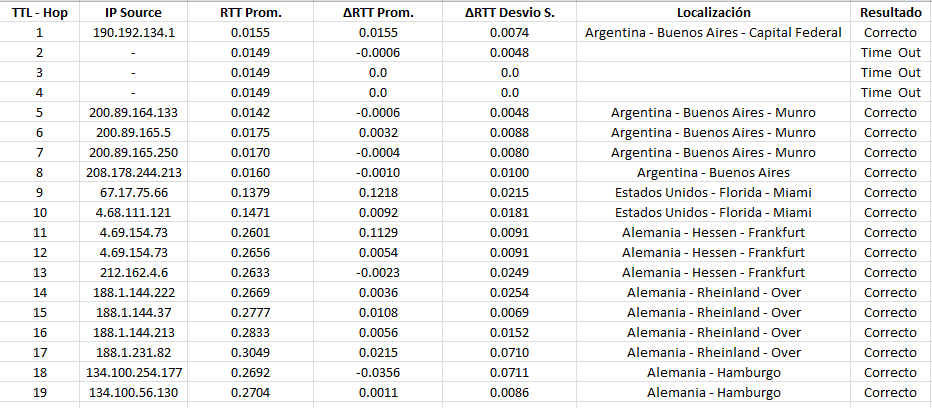
\includegraphics[width=1\textwidth]{img_analisis3/captura.png} 
	\end{center} 
\end{figure}
\vspace{0.25cm}

\subsubsection{An\'alisis de los resultados}
Mediante gr\'aficos haremos un an\'alisis de los resultados obtenidos. \newline


\begin{figure}[h]
	\begin{center}
    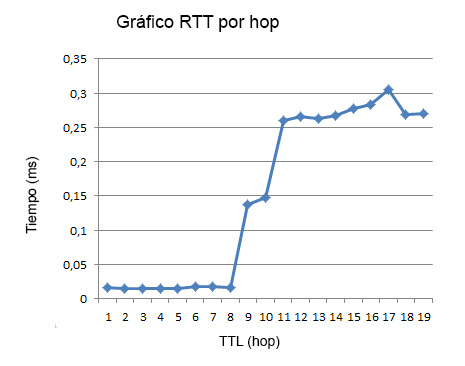
\includegraphics[width=0.5\textwidth]{img_analisis3/grafico-rtt-promedio.jpg} 
    \caption{$RTT$ promedio - Universidad de Hamburgo}	
	\end{center} 
\end{figure}
\vspace{0.25cm}

\begin{figure}[h]
	\begin{center}
    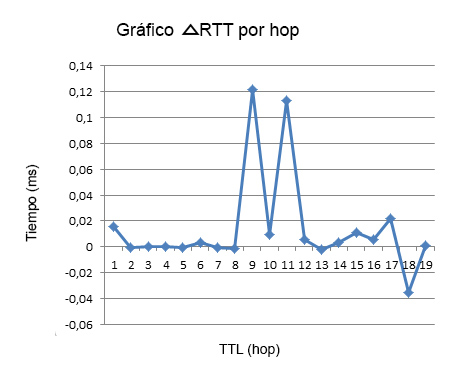
\includegraphics[width=0.5\textwidth]{img_analisis3/grafico-delta-rtt-promedio.jpg} 
    \caption{$\Delta RTT$ promedio - Universidad de Hamburgo}	
	\end{center} 
\end{figure}
\vspace{0.25cm}
%\newline
\newpage

De la muestra obtuvimos que los $\Delta RTT$ sigen una distribuci\'on Normal y que los enlaces submarinos, según los outliers obtenidos mediante el test de Grubbs, se corresponden con el salto 9 y el 11.\\

Podemos notar en el gráfico RTT por Hop, que habla de los RTT promedio de cada salto, una gran subida de tiempo del Hop 8 al 9 y del Hop 10 al 11. Entre los Hops 16, 17 y 18, se logran unos intervalos de tiempos un poco mayor al resto de los saltos, aunque sin ser muy relevantes.\\

En el segundo gráfico $\Delta RTT$ por Hop, que habla del tiempo expecifico que consume cada salto con su antecesor, se aprecia dos picos muy pronunciados en el Hop 9 y el Hop 11. Asi mismo, como mencionamos en el primer gráfico, aca también se aprecian unos picos no tan pronunciados del Hop 16 al 19.\\

Analizando los dos gráficos y viendo los datos que tienen en común, podemos notar que los hops más distinguidos, corresponden a los detectados por nuestro test de grubbs como outliers. Esto tiene mucho sentido dado que buscamos enlaces submarinos, o sea con distancias física muy grande.\\

Al observar la geolocalización aportada por nuestra página web, para cada IP de los saltos, notamos que: del hop 1 al 8 se mantiene en Argentina, del hop 9 al 10 en Estados Unidos y del 11 al 19 en Alemania. Podemos apreciar además que los Hop detectados por el test de Grubbs corresponden efectivamente a enlaces submarinos, dado que en el hop 9 pasa de Argentina a Estados Unidos y en el hop 11 pasa de Estados Unidos a Alemania, cambiando de continente en este último. Cabe mencionar la gran eficiencia de nuestro geolocalizador usado en este exprimento que es diferente a los experimentos anteriores, y nos aportó información mucho más acertada que en las muestras anteriores.\\

%Al observar los gráficos podemos notar que los resultados obtenidos mediante el test de Grubbs son correctos, ya que del salto 8 al 9 el paquete enviado viaja, según la geolocalización de las IP, desde Buenos Aires a Miami y su RTT promedio aumenta significativamente, y del salto 10 al 11 el paquete viaja de Miami a Frankfurt donde también hay un cambio abruto de su RTT promedio.\\
%No hay mucho para analizar en esta experimentación, dado que el test de grubbs se logra contrastar con la geolocalización detectada por nuestra página web. Lo cual nos habla, a diferencia de los experimentos anteriores, que
%\\
Finalmente presentamos un mapa global donde vamos a trazar los puntos importantes de la ruta que realizan los paquetes. 

\begin{figure}[h]
	\begin{center}
    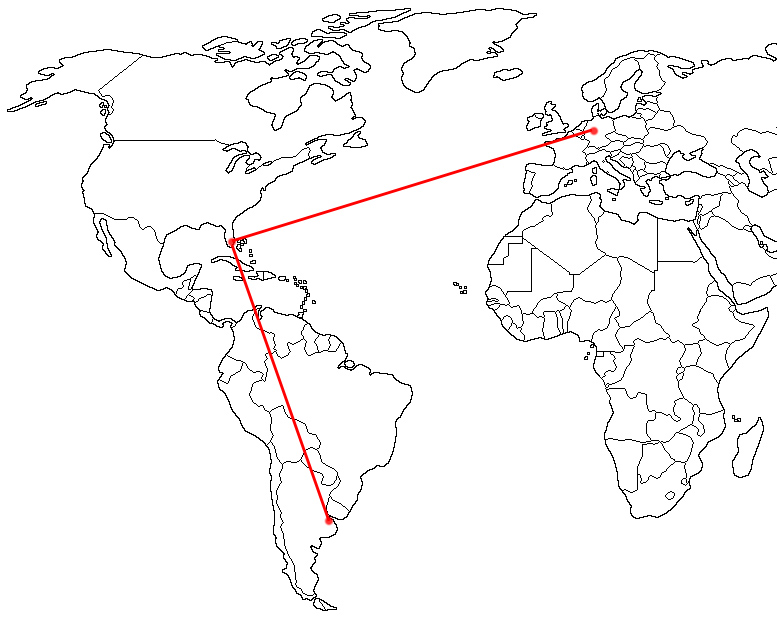
\includegraphics[width=0.7\textwidth]{img_analisis3/mapa.jpg} 
    \caption{Figura 1: Ruta del paquete - Universidad de Hamburgo}	
	\end{center} 
\end{figure}
\vspace{0.25cm}